\chapter{相关概念}

% 7-9 页


\section{广域互联网络的路由架构}

\subsection{广域网络的结构组成}

广域网是横跨国家、地区的、相互连接的全球性网络系统,如此庞大的体系决定了它必定将使用分布式的方式组成和管理,参加广域网络的组成部分依照一定的规则交换确认彼此的身份,并同时交换路由信息\citing{douzet2020measuring}。

\subsubsection{基本组成与管理方式}

互联网的基本组成单元是其中的成员网络,它们是能够被是作为一个行政实体的,一组或一个处于相同或类似策略管理下的路由器和终端设备,被称为自治系统(AS)。自治系统内部通过内部网关协定(IGP)交换系统内部的路由条目,而数以万计的自治系统相互独立建立自己的连接,并通过外部网关协定(EGP)在广域网层面交换彼此整个系统的路由项目,其中边界网关协定(BGP)是广域网络中唯一公认的外部网关协定\citing{rekhter2006border},因此后续的路由异常问题分析均以 BGP 协议为基础进行。

与通过 IP 地址确定设备的网络地址类似,BGP 协定使用一种称为自治系统编号的唯一标示符来确定一个自治系统的身份,它的范围是4个字节(0-4294967295)\citing{rekhter2006border}。在互联网中,互联网号码分配局(IANA)负责管理这些号码及所属于这些自治系统的 IP 地址的的分配,它通过一种层次结构将这些资源分配给五个区域互联网注册局(RIR),而这些注册局则通过本地互联网注册局(LIR)向下分配获取的资源和网络号码\citing{angieri2019distributed}。

\subsubsection{商业网络的层次结构}

在互联网中,路由信息的传递并不一定是无方向的。在实际的互联网络中,大部分具有较多直接连接或具有更优质线路的网络是商业公司,它们将向具有更低连接性的网络及其客户网络提供付费的连接服务,这直接体现在了路由信息的传递上,在与网络路由相关的研究中,这类单向的信息传递通常被称为非对等互联(Transit)\citing{gregori2011bgp}。

由于上述原因,互联网的路由结构从最初设计的完全分布式逐渐地转变为了具有了一定层次和中心性的结构\citing{vanbever2009hierarchical}:一些网络能够经由更少的自治系统,从而抵达互联网的每一个角落,它们被认为具有更高的中心度。

因而,有研究提出了“客户锥形”的概念\citing{luckie2013relationships}:一个自治系统的客户锥形是它自身和在广域网中能够观察到的通过非对等互联路由可以到达的所有AS,即它和它的任意阶客户。

% 来个公式

对于一个自治系统而言,位于它的客户锥形中的自治系统的路由一般会直接或间接地经由它,因而这项指标展示了它对网络资源的控制能力\citing{luckie2013relationships},即能够影响到网络中的哪些部分的路由。在一些研究中,它的大小常常被用作一种衡量标准,用于度量自治系统的相对规模\citing{doverspike2010structural}。

与此同时,一些网络常常还会与其它网络建立互利且双向的路由交换,相互直接交换各自的路由信息,通常任何一方都不向对方支付费用,这种关系被称为对等互联(Peering),通常这类对等路由不会继续发送给对等方以外的自治系统。\citing{vanbever2009hierarchical} \citing{luckie2013relationships} 在一些被称作互联网交换点的设施内,会有大量 AS 形成近似于全连接(Full Mesh)的对等互联关系,据调查显示,对等互联大大降低了流量结算成本,并降低了互联网日益提升的中心度\citing{luckie2013relationships}。

\begin{figure}[h]
    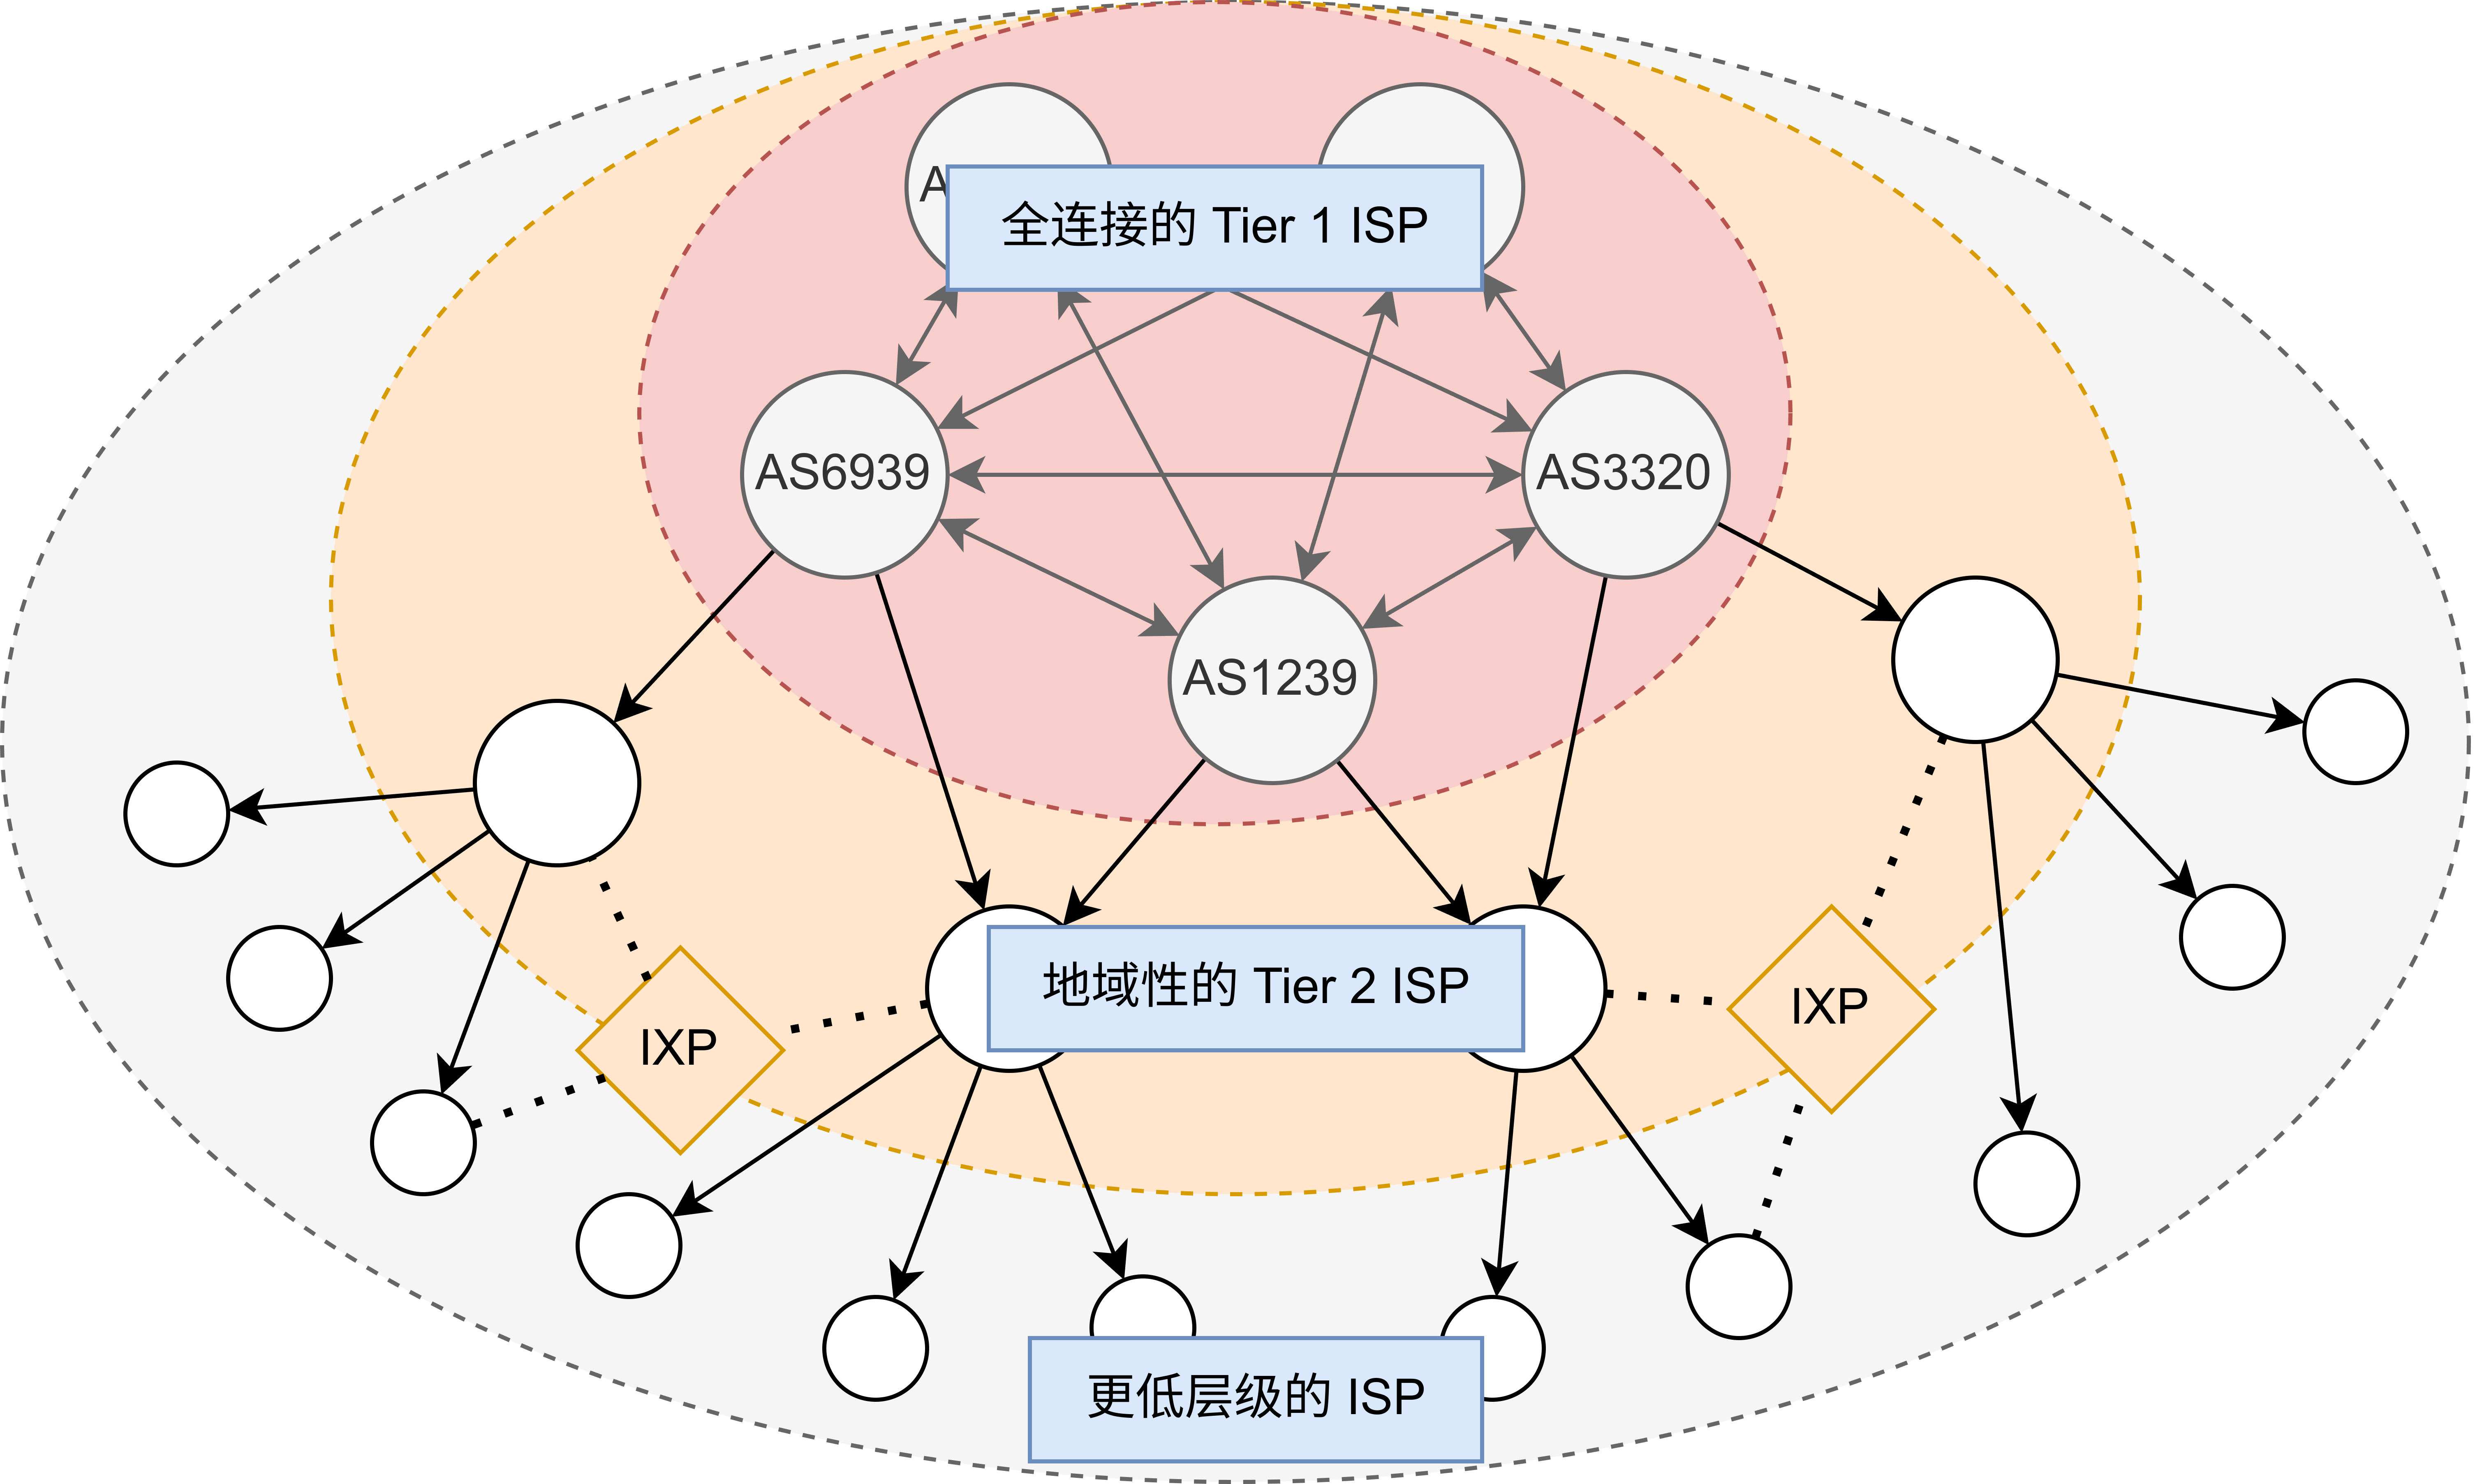
\includegraphics[width=0.7\linewidth]{chapter/c2_images/c2_wan-asn-structure.png}
    \caption{广域网络的层次结构}
    \label{c2_wan-asn-structure}
\end{figure}

图 \ref{c2_wan-asn-structure} 更加直观地展示了互联网中存在的三级层次结构\citing{doverspike2010structural}:彼此相互全连接(Full-Mesh)提供非对等互联路由(事实上即是全部网络路由)的I类自治系统(Tier 1);直接由I类自治系统提供非对等互联路由的II类自治系统(Tier 2);间接通过上级自治系统访问全部网络的III类自治系统(Tier 3);这些自治系统还直接或通过互联网交换点间接进行对等路由的交换。

\subsubsection{分布式网络的对等结构}

在互联网之外,还存在一些社区维护的实验性分布式网络\citing{mirz2018distributed},它们的大部分网络通常是双向提供非对等互联服务的,即在对等互联会话中交换全部已知路由,因此在结构上具有截然不同的特点,例如由于不存在商业关系,整体上具有更少的中心度、成员自治系统的组织一般不具有层次性。

中国教育和科研计算机网(China Education and Research Network,简称 CERNET)\citing{li2011china}是我国教育部、赛尔网络与众多国内高校合办的实验性网络。虽然 CERNET 本身是互联网的参与方,但它的成员单位大多拥有自己的自治系统号码,并相互通过 BGP 协议交换自身的路由,因而在内部能够被视作为一个分布式广域网络。

DN42(Decentralized Network 42)\citing{dn42us}是一个由社区发起的的去中心化网络。 与一般的网络不同的是,DN42 拥有着与其他网络相独立的地址空间、自治系统编号规则和域名系统,因此其架构完全独立于互联网,并且其参与方通常使用重叠网络(Overlay Network)技术,通过底层网络建立网络隧道与其它自治系统相互连接,而非借助光纤或网线的方式通过物理介质连接,这样的组网方式降低了网络的申请门槛,因而在尺度上具有一定的规模,适合用作网络相关研究。

\subsection{广域网络中的路由协议原理}

由于 BGP 协议在自治系统间的广泛性和通用性,广域网络中的路由在通常情况下指使用 BGP 协议在广域网中交换的路由,它与内部路由协议不同,不使用常见的最短路算法,而是让每一个自治系统保留一份当前视角的全球路由表,并直接根据路由表中的属性选择路由\citing{rekhter2006border}。以下将介绍它的基本原理。

\subsubsection{路由信息交换}

由于广域网的分布式和开放性,使得它的路由不存在用于统一调度和管理的中心机构,这使得它具有强大的纠错能力。即使自治系统之间没有直接连接,或是直接连接因故断开,边界路由协定会帮助路由器寻找替代路径,虽然可能在传输延迟、带宽等受到限制,但是仍然能够正常通信\citing{verma2018analysis}。总的来说,互联网的分布式系统理论上是具有良好的鲁棒性的。

自治域内通过内部路由协定交换的域内路由通常不会传播到自治域外,并且具有更少的层次结构,而由于处于统一管理之下,网络拓扑结构上的变化是可预测的,因而此类路由一般不会出现异常。而每个自治域之间的路由则由自治域间的链路状况、主机状况,甚至是政府的监管审查、贸易壁垒等非技术因素而决定,所有自治域共同组成分布式系统,互联网这一整体将随着各节点的情况改变而不断改变自身的拓扑结构,位于自治域之间的、通过边界路由协定交换的域间路由也将随之变化\citing{al2016bgp}。因为其路由条目属性过多、路由选择策略较为复杂,常常因为外界因素出现异常状况。

\subsubsection{路由选择算法}

与统一管理的内部路由协议不同,为了保证路由系统的所有参与者都能够自行决定最优路径,BGP 协议要求路由条目中的属性信息尽可能地能携带自定义的字段,并被任意途径的自治系统说采用。

% 总的来说,它包含四种类型的属性信息:

% \begin{enumerate}
%     \item 众所周知的强制属性:所有自治系统的路由器都能识别并处理,并且字段必须被包括在传递的每一条路由信息中。
%     \item 众所周知的可选属性:所有自治系统的路由器都能识别并处理,字段能够可选地被包括在传递的路由信息中。
%     \item 可选的传递性信息:能够被一些自治系统的路由器识别并处理,即使不能识别,也需要被包括在进一步转递出去的路由信息中。
%     \item 可选的非传递性信息:能够被一些自治系统的路由器识别并处理,它们能够被忽略掉,不被包括在进一步转递出去的路由信息中。
% \end{enumerate}

以下是协议中最常见的两种属性信息,它们将在后续章节的研究中使用:

\begin{enumerate}
    \item 自治系统路径(AS Path)\citing{rekhter2006border}是一种强制编码在路由条目中的信息,它表达了路由在自治系统层面的传递信息,可以被理解为一条由节点 ID(自治系统编号)组成的有向路径。每个自治系统在将路由信息转递前,都会在此路径的首部添加自己的AS号码,以防止路由循环。
    \item 社区(Community)\citing{donnet2008bgp}是一类可选的信息,它能够理解为这条路径所关联的标签,这类标签信息既可以是私有的(只在某些自治系统有效)也可以是共有的(一些预定义的属性会在所有自治系统生效),路由消息在传递的时候,自治系统的路由器能够根据规则去添加、删除和改写这些标签。
\end{enumerate}

与内部网关协定中复杂的权重不同,由于自治系统之间难以统一协调,加之过于巨大的网络拓扑使得精确的路径寻找较为困难,一般情形而言,广域网的 BGP 协议寻路使用最短自治系统路径,同时使用社区属性对一些需要特殊优先级的路由进行调整。

自治系统路径能够反映出路由中的拓扑信息,而社区属性是对整个路径的标签信息,通过这两个信息能够构建出一个有向带权重的图。由于其它信息在不同自治系统下具有不同的数值定义,因而无法仅通过数据集确定意义,故无参考价值,本文不再介绍。



\section{广域网络路由异常}

\subsection{路由协议的固有缺陷}

广域网络的路由事实上是非常脆弱而易受攻击的。实际上,BGP 最初被提出以来,没有任何被协议所直接包括的安全机制\citing{mitseva2018state},路由的稳定可靠完全是基于网络运营商之间的信任和恰当的设置,也即假定系统永远不会出现随机故障或安全问题,路由器之间不会发送错误的数据。这引入了一个明显的漏洞:如果路由协议的其中某个参与方出于恶意,试图通过BGP协议影响其它自治系统乃至全球的路由表,其它的自治系统没有任何通用的手段来阻止它的发生。

在 1998 年,RFC2385 对 BGP 引入了密码保护机制\citing{heffernan1998protection},解决了通过二层链路劫持 BGP 会话的可能性,但它使用易受攻击的 MD5 加密,至今尚未更改。1999 年,RFC2439 对 BGP 引入了路由震荡抑制(Route Damping)\citing{villamizar1998bgp}机制,缓解了 BGP 的路由震荡问题。然而,在标准提出的几十年来,广域网络上的路由异常问题从来没有得到根除,究其原因有二:

其中一个原因是针对底层协议和标准的修改难以被普遍采纳。一项报告指出,互联网运营商的核心设备的更新周期长达 10-15 年,并拥有相当大的方差\citing{mahimkar2010detecting},这意味着在新的标准提出后,大部分设备都很难短时间内进行引入\citing{mitseva2018state},或是为了与其它互连的运营商兼容的原因关闭这些增强安全性的功能。

另一个重要原因是,这些手段事实上并未解决来自恶意的路由协议参与者和不遵循规范的配置者的安全威胁\citing{sermpezis2018survey}。基于信任的广域网架构仍然坚持默认所有路由参与者不会存在恶意破坏的可能性,这是维持互联网分布式的基础。

因而,由此产生的安全性问题,包括路由异常问题,便从标准性问题转变为了无法避免的问题,它的潜在安全威胁使得对路由系统的安全性的建模研究更具意义。

\subsection{广域网络的潜在安全威胁}

% \subsubsection{路由震荡}

% 路由震荡是指由于物理故障、系统错误、人为因素等原因,所造成的路由表的频繁变化。相互连接的分布式网络会因此不断向相邻自治系统宣告和撤回路由,导致其他节点频繁重新计算路由。这会对整个网络造成严重的算力和链路负担,轻则网络延迟升高、不稳定,重则导致拒绝服务攻击(Denial of Service,DOS),并造成大规模的网络服务瘫痪。

% 这样的问题可以通过修改外部网关协议的行为,来防止系统资源的枯竭,例如在 BGP 协议中启用路由震荡抑制功能,临时关闭反复路由更新的邻接系统的 BGP 会话,或是限制对应协议的更新频率。

% \subsubsection{路由劫持}

路由劫持是广域网中最常见的安全威胁。当一个自治系统因为配置错误或恶意行为的情况下,它会宣告并不应由它宣告的路由条目,如果它的邻接系统没有部署 RPKI 机制或是没有强制启用路由的过滤机制,这些错误的路由条目就会通过 BGP 会话传播到它的邻接系统,并进而被发送至整个广域网内所有可达的边界路由器中,这时候路由劫持事件即被触发,由于 BGP 路由协议的规则影响,目的地涉及到被劫持的 IP 地址块的网络流量有可能会被路由至发起劫持的自治系统\citing{mitseva2018state}。而现代互联网的系统反应时间非常迅速,根据一项调查显示\citing{sermpezis2018survey},被劫持的路由条目能够在 10 秒时间内抵达全球 90\% 以上的互联网系统。

并非所有的 BGP 劫持都能够成功造成安全危害,事实上,对网络的拓扑结构造成更大影响的 BGP 劫持通常能有能力影响更多或具有更大客户锥形的自治系统,这通常有两种方式:

\begin{enumerate}
    \item 发起劫持的自治系统宣告前缀长度更长的路由。网络系统的路由层次性决定了路由器在接收到更准确的IP地址块的路由信息的时候,会直接采用并完全弃用任何路径选择算法。
    \item 提供更为直接的自治系统路径,利用广域网路由选择算法的特点,构造出比正常路由更短的自治系统路径,这将使得路由器认为该路由在逻辑上更优。
\end{enumerate}

% 大型网络或网络群的运营商(其中很多是ISP)会明目张胆地进行这种恶意活动,这似乎令人惊讶。但考虑到据统计,现在全球有超过8万个自治系统,有些自治系统不值得信任也就不足为奇。此外,BGP劫持并不总是那么明显或容易被发现。坏人可能会把他们的活动伪装在其他自治系统的后面,或者宣布一些不可能被注意到的未使用的IP前缀块,以便不被发现。

图 \ref{bgp-hijack} 显示出了一种典型的基于更长前缀的路由劫持,AS3 通过向广域网宣告 1.14.5.0/24 这一更长的路由前缀,劫持了本应属于 AS1 的 1.14.0.0/16 的路由,并将访问 1.14.5.14 IP 的流量引导向攻击者的设备,整个流程中 AS1 及其 AS2 没有执行任何错误操作,同范围的其他 IP 也能通过一种称为流量穿透的方法返回正常目的地,从而实现隐蔽的攻击手段。

一些网络运营商可能因为配置失误,将内部或错误的路由发送至自治系统外,造成BGP劫持,这样的情况常常被称为路由泄露,据调查,此类事件相比于恶性的劫持事故而言往往更加常见\citing{vervier2015mind}。根据一项研究显示,并不是所有的 BGP 劫持事件都能够被注意到并及时采取措施\citing{schlamp2016heap},攻击者可以选择不常使用的地址块,或是未被注册的地址块进行劫持。以上原因都导致了路由异常的检测实质上难以判断是否是恶意攻击行为。

\begin{figure}[h]
    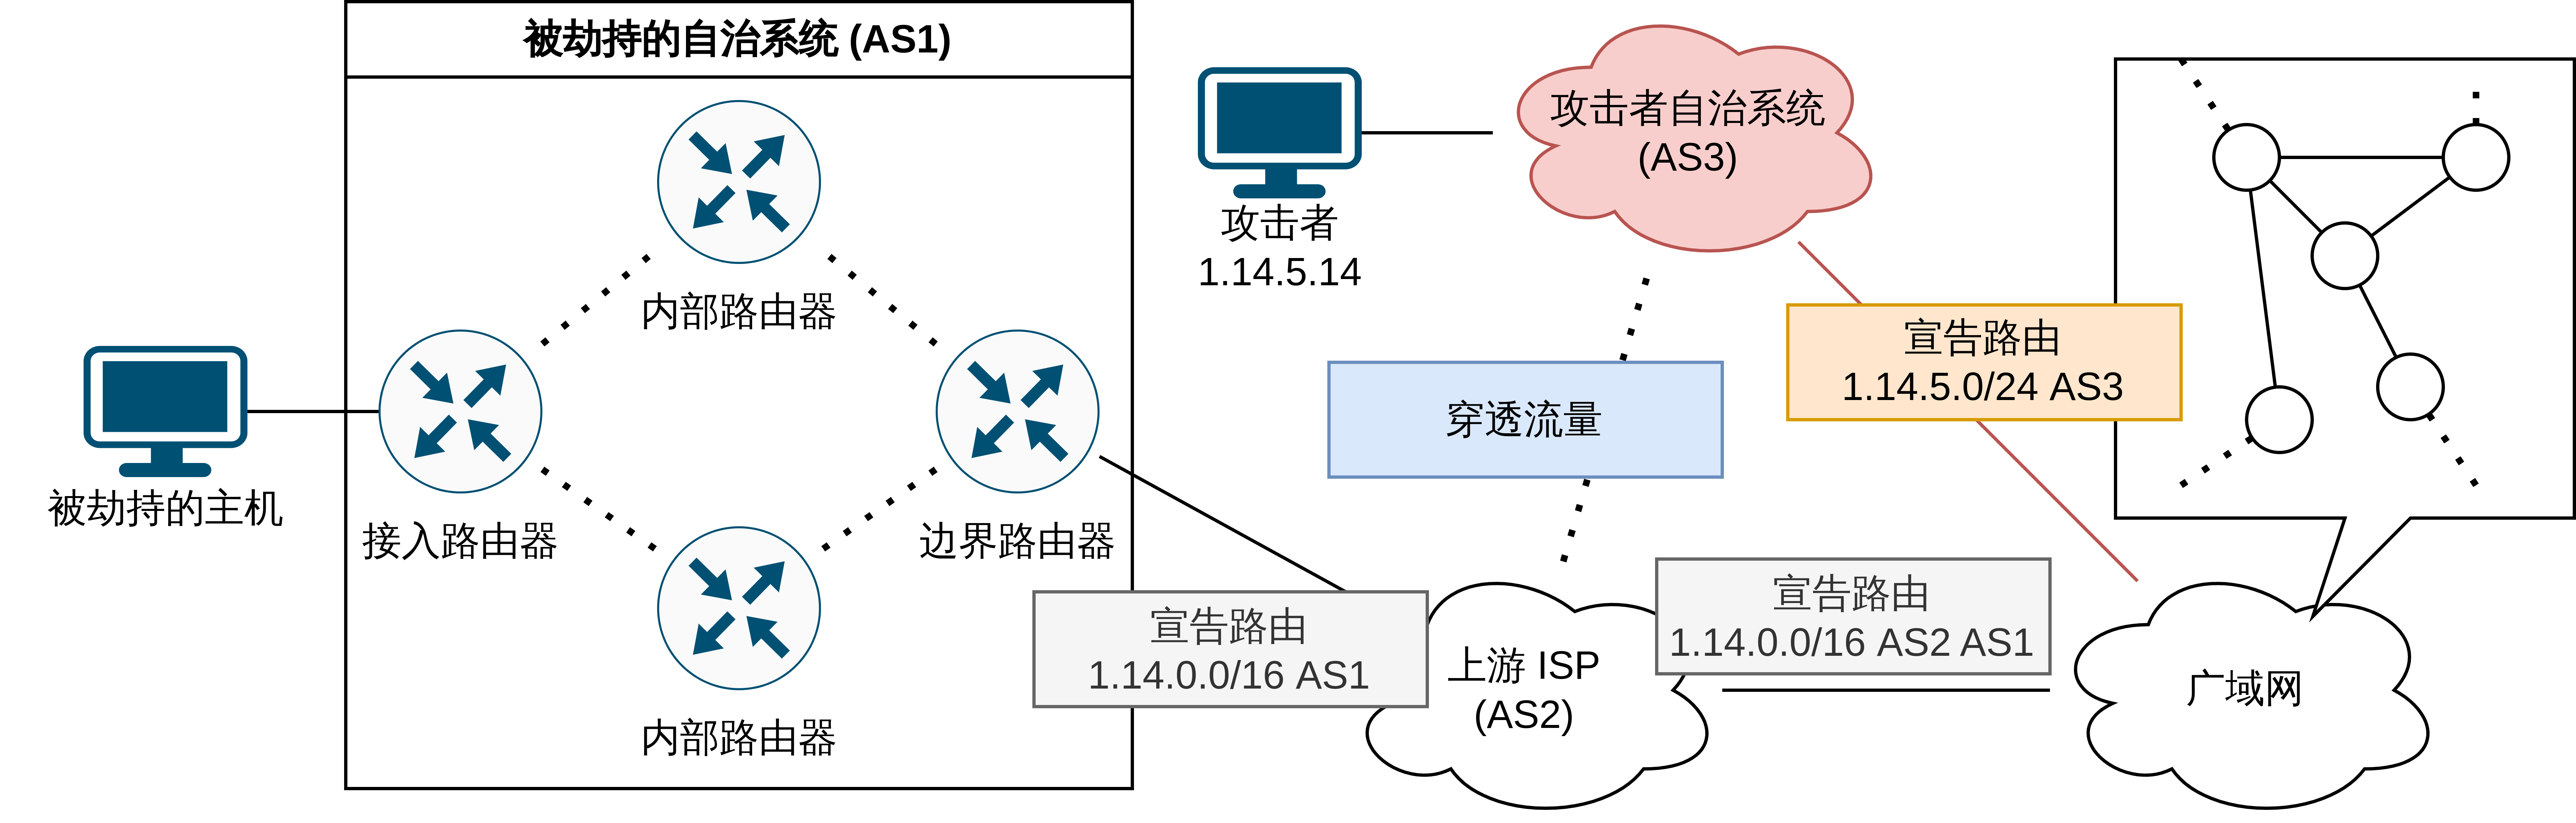
\includegraphics[width=\linewidth]{chapter/c2_images/c2_hijack.png}
    \caption{BGP劫持示意}
    \label{bgp-hijack}
\end{figure}

\subsection{路由异常的定义}

路由异常,被定义为一种表现出异常特征的路由更新条目,它通常携带有异于其它正常路由拓扑的自治系统路径,并有可能在其它属性上呈现出不同的特点\citing{al2016bgp}。它一般包括两类状况,一种是 BGP 劫持,这类事件通常是有害的;而另一类是新路由的增加,由于分布式网络的系统之间常常建立和断开连接,这一类异常状况既可以是突发事件,也可以是可预测的人为因素,它们并不会产生实质性危害。

由于现有数据集中基于图网络的有标记路由异常事实上并不多见,此类问题一般被认为是一种无监督学习问题。

\subsection{问题的图网络表述}

% 使用基于图网络的数学公式描述问题。
下面通过图网络的数学语言描述本研究所定义的广域网络异常检测:

对于一条路由 $R_i$,它包含三种属性,即对应的 IP 前缀 C,AS 路径 P,社区信息 C,即 $R_i = \{ O, P, C \}$,它们共同组成全球路由表 $R_T = \{ R_i \}$。
% 全球路由表 {R_i} , R_i = {O(前缀), P(路径), C(社区)}

前缀 C 是一个标识符;AS 路径 P 可理解为一个不定长的有序列表 $P = \{A_1,A_2..A_N\}$,其中,路由的源自治系统指宣布该路由的自治系统,对应列表中的最后一个元素 $A_N$;社区信息 C 是一个标签集合 $C = \{C_1,C_2...C_N\}$。

% last(P) = origin

定义图生成算法 $f_g$ 为从路由表数据构造图网络数据集的方法,具体来说,$f_g(R_T)=G<V,E>$,其中节点集 V 是路由表 ${R_i}$ 中所有路由路径上的自治系统号码,即 $V = \forall(A_i \in P \in R_i)$,该算法通过 $R_i$ 特征生成一个有向或无向图 $G<V,E>$,它的边集 E 将由算法 $f_g$ 决定。
% 图生成算法 f_g({R_i})=G<V,E> V=all(P)

定义图嵌入算法 $f_e$ 为从图网络数据 $G<V,E>$ 中提取嵌入数据的方法,它对于每一个图元素输出一个 k 维向量嵌入,即 $e = f_e(G<V,E>) = \{ e_i \}$,而图元素可以是图上的所有节点,也可以是边集或是路径集,即 $N = len(V/E/R)$。
% 嵌入算法 e = f_e(G<V,E>)={e_i} N=num(V/E/R)

最后定义异常分数 $f_a$ 是由新的路由和原有的图数据及其嵌入作为输入,输出对更新路由的异常分数以便于最终进行异常检测,即 $f_a(R_n,G<V,E>,e) \in (0,1]$。
% 定义异常分数 f_a(R_n,G<V,E>,e)

广域网络的路由异常检测问题的本质即包含了以下的部分:

\begin{enumerate}
    \item 设计图生成算法 $f_g$,将原网路数据集转换为图数据集。
    \item 设计高效的嵌入算法 $f_e$,将图数据集转换为图元素的嵌入。
    \item 定义异常检测分数 $f_a$,用以检测新的测试样本。
\end{enumerate}


\section{图网络的嵌入算法概述}

由于图网络数据一般具有大量的节点,通常具有较高的维度,因而很难被传统的基于特征的方法处理。而已有的研究证明,节点的低维嵌入在较大规模图网络中,能够作为较好的特征输入,例如节点分类、链路预测和异常检测\citing{cai2018comprehensive}。

图嵌入算法即成为了降低网络维度,并解决该问题的一种方式。图嵌入算法的基本思路是将网络中的节点特征嵌入到维度更低的空间中,并保证在压缩后的向量空间中,相似的节点依然能够更接近,即尽可能保留拓扑的相似度关系。

以下是一些图网络的嵌入算法的概述,它们将在后续研究中被使用到。

\subsection{图的嵌入}

首先介绍图的嵌入的定义。对于一个图而言,它的嵌入是指它的元素的映射。具体而言,对于一个图 $G<V,E>$ 而言,它的节点嵌入是它顶点的映射关系,如公式 \ref{graph_embedding} 所示:
\begin{equation} \label{graph_embedding}
f:v_i\rightarrow y_i \in R^d, \forall i \in [n]
\end{equation}

图的嵌入算法 f 能够保证节点属性在将维度降至 $d(d<<n)$ 的情况下依然能够保留节点之间的相似度关系。同时,也能够通过类似的过程,将图的其它元素(边、路径等)转化为低维向量。

\subsection{GraphSAGE 模型}

GraphSAGE 模型\citing{hamilton2017inductive}是为了解决经典图卷积网络需要大量图数据输入、无法实现归纳学习等特点而提出的特征聚合方法。在介绍 GraphSAGE 模型前先介绍图卷积网络的概念。

\subsubsection{图卷积网络}

图卷积神经网络\citing{kipf2016semi}是一种图嵌入方法,它的主要目标是通过消息传播和更新的方法,使用多个图卷积函数(即多个卷积层),学习一个图卷积函数,用以将自身和邻居的特征聚合,并输出节点的表示。

然而,传统的 GCN 模型在面对大规模数据集上存在诸多问题\citing{gao2018large}。首先,GCN 的嵌入算法涉及到对整个图的特征矩阵进行多层变换,这意味着它自身具有较高的复杂度;其次,训练 GCN 无法实现归纳学习,在每一次模型更新时都需要对整个图进行重新计算。

\subsubsection{基本结构}

而 GraphSAGE 模型是一种利用采样和聚合节点特征,进而实现归纳学习的图网络算法。它的基本思路是利用已有的拓扑信息,对节点的邻居进行采样,并通过聚合函数的方式,将高阶的邻居信息在不同层次上进行聚合,从而得到最终的嵌入,并用于下游任务。

GraphSAGE 通过以下方式进行迭代,从而获得节点的高阶嵌入:
\begin{equation} \label{graphsage_iter_aggr}
h^k_{N(v)} \leftarrow AGGREGATE_k(\{ h_u^{k-1}, \forall u \in N(v)\})
\end{equation}
\begin{equation} \label{graphsage_iter_concat}
    h^k_v \leftarrow \sigma(W^k \cdot CONCAT(h_v^{k-1}, h^k_{N(v)}))
\end{equation}

它首先依照公式\ref{graphsage_iter_aggr}对节点 v 的邻居的 $(k-1)$ 层嵌入进行聚合,然后按照式\ref{graphsage_iter_concat}中的方法与自身 $(k-1)$ 层特征拼接从而得到第 $k$ 层的特征。它在无监督学习下使用针对邻居的对数近似和针对非邻居的负对数近似使得相邻节点尽可能拥有相同的嵌入。

在GraphSAGE模型中,$AGGREGATE$ 即聚合函数\citing{hamilton2017inductive}是最重要的部分,它决定了如何结合采样到的邻居节点的特征。关于聚合函数的选择有两个条件:

\begin{enumerate}
    \item 可导,因为要反向传递来训练目标的聚合函数参数。
    \item 对称,这里的对称指的是对输入不敏感,因为在聚合的时候,图中的节点关系并没有顺序上的特征。
\end{enumerate}

\subsection{随机游走和图嵌入}

\subsubsection{图网络的随机游走算法}

随机游走\citing{pearson1905problem}是一种典型的基于图网络的采样过程,它被定义为一种以特定随机分布在图网络上选取路径的方式。随机游走的输入是一个图 $G<V,E>$,输出一个路径的集合 $\{ P_i|P = Random\_Walk(G) \}$。随机游走的采样规则可由公式\ref{markov_chain}给出,它实质上是一种有限马尔可夫链:
\begin{equation} \label{markov_chain}
p_{t+1}(a) = \sum_{b:(a,b)\in E} \frac{\omega(a,b)}{\Sigma_{a}\omega(a,b)} p_t(b)
\end{equation}

其中,它包含一个用以根据当前信息(图 G 及其节点 V 边 E 的某种度量值及其组合)决定转移概率的 $\omega$ 函数。

\subsubsection{基于 node2vec 的节点表征 和 基于 path2vec 的路径表征}

在通过随机游走获得采样路径后,即可根据这些路径来生成节点的表征。node2vec \citing{grover2016node2vec}即是一种采用此种方法的节点嵌入模型。

在自然语言处理中,基于语句的 Skip-gram 和词袋的 word2vec 模型被用于对句子中的词语进行建模。node2vec 模型则假设图中的节点可以被视作为可用词语的全集,对节点的路径采样能够体现出图的拓扑结构,正如对词语的组织能够体现出语义信息一样。受此启发,将随机采样的路径送入文本挖掘的嵌入模型中能够很好的反映出节点的拓扑特性 \citing{grover2016node2vec}。

path2vec \citing{kutuzov2018learning} 是对 node2vec 模型的拓展,也是 doc2vec 模型在图网络中的对等模型,它拓展了 node2vec 的采样方式,通过预定义的图距离度量方式对节点进行嵌入,进而能够学习到比 node2vec 更加高阶的拓扑结构关系。


\section{图网络的中心度度量}

在图网络中,中心度\citing{rodrigues2019network}是一种很重要的指标,它用以衡量图网络节点在图中以某种度量方式下的重要性或权重。

在图论中,有许多用于衡量图中心度的指标,它们反映了数据集在不同角度上的特征信息。常用的中心度指标有:

\begin{enumerate}
    \item 度中心度(Degree Centrality):一个节点的度中心度是指该节点在网络中所连接的边数或者连接的节点数。该指标通常适用于基于传播效率的场景。
    \item 距离中心度(Closeness Centrality):一个节点的距离中心度是指该节点与其他节点之间的距离之和的倒数。该指标通常适用于基于连接紧密程度的场景。
    \item 介数中心度(Betweenness Centrality):一个节点的介数中心度是指该节点在所有最短路径中出现的频率。该指标通常适用于基于促进整个网络的连接程度的场景。
    \item 特征向量中心度(Eigenvector Centrality):一个节点的特征向量中心度是指该节点与其他节点之间的连接强度的加权和。该指标通常适用于度量节点的相似程度。
\end{enumerate}

通常情况下,在基于路由的互联网络中,介数中心度\citing{liu2013characterizing}更具实际意义,它能够反映对应的网络节点在路由中的控制力和重要性。

\section{本章小结}

本章节主要介绍了本文涉及到的相关技术概念和主要研究内容。在 2.1 节,介绍了广域网络的基本组织结构,是后续章节中涉及拓扑构建的模型的技术基础。本章在 2.2 节引入了路由异常的背景概念和原理,并通过图网络的角度对问题进行了表述。在 2.3 节中,本章还介绍了后续研究将使用到的一些嵌入算法。最后,本章在 2.4 节对图的中心度这一重要度量指标进行了初步介绍,并针对随机游走介数中心度的意义进行了阐述,这项指标在后续章节中被广泛使用。